\documentclass[10pt,twocolumn,letterpaper]{article}
\usepackage[utf8]{inputenc}
\usepackage[T1]{fontenc}
\usepackage{mathptmx}
\usepackage[margin=0.78in]{geometry}
\usepackage{amsmath,amssymb}
\usepackage{booktabs}
\usepackage{graphicx}
\usepackage{hyperref}
\usepackage{xcolor}
\usepackage{caption}
\hypersetup{colorlinks=true,linkcolor=blue,citecolor=blue,urlcolor=blue}
\setlength{\columnsep}{0.28in}

\title{\Large \textbf{OdiaSLM: From-Scratch Pretraining, Morphology-Aware Tokenization, and Calibrated Evaluation of 60M and 100M Small Language Models for Odia}}

\author{
  \textbf{Arun Misra} \\
  AI Researcher \\
  Bhubaneswar, Odisha, India \\
  \texttt{\href{https://huggingface.co/arunjmisra2273}{huggingface.co/arunjmisra2273}} \\[3pt]
  \small \textbf{DOI:} \texttt{\href{https://doi.org/10.5281/zenodo.24167433}{10.5281/zenodo.24167433}}
}
\date{November 12, 2026}

\begin{document}
\maketitle

\begin{abstract}
While frontier multilingual Large Language Models (LLMs) achieve remarkable capabilities on high-resource languages, they impose a severe ``tokenization tax'' on morphologically rich, low-resource Indic scripts such as Odia (\textit{ory\_Orya}), fragmenting words into 5--6$\times$ more subword tokens than English and inflating inference latency. We present \textbf{OdiaSLM-60M} (62.11M parameters) and \textbf{OdiaSLM-100M} (100.69M parameters), two sovereign decoder-only Small Language Models pre-trained from scratch for Odia on up to 1.57 billion tokens drawn from a strictly deduplicated and 13-gram benchmark-decontaminated corpus of 9.62 million documents (1.247 billion words). First, we design a 16,384-vocabulary canonical NFC-normalized SentencePiece BPE tokenizer that preserves Odia \textit{juktakshara} conjuncts, achieving a fertility of \textbf{1.4809 tokens/word} (11.57 UTF-8 bytes/token), 0 \texttt{<unk>} tokens, and a 3.6$\times$ compression advantage over general multilingual tokenizers. Second, utilizing Grouped-Query Attention (GQA), SwiGLU, Half-Split RoPE, FP32-variance RMSNorm, auxiliary Z-loss stabilization, a Warmup-Stable-Decay (WSD) schedule, and two-stage context extension ($512 \rightarrow 1024$), we demonstrate clean neural scaling from 62.11M (validation perplexity \textbf{19.92}, Bits-Per-Byte \textbf{0.3965}) to 100.69M parameters (validation perplexity \textbf{17.14}, Bits-Per-Byte \textbf{0.3767}, Top-1 token accuracy \textbf{44.61\%}). Third, we conduct a comprehensive zero-shot evaluation across 27 tasks in the Odia Evaluation Benchmark, uncovering both cross-lingual untranslated choice artifacts in 9 tasks and severe surface-form competition under raw log-likelihood. Applying Pointwise Mutual Information (PMI) calibration unlocks a macro-average accuracy of \textbf{60.83\%} across the 18 pure-Odia benchmarks (\textbf{+34.44\%} lift over random chance). Both models are released in native \texttt{LlamaForCausalLM} format under a dual non-commercial and commercial license.
\end{abstract}

\section{Introduction}
Odia is a Classical Indo-Aryan language spoken by over 45 million people, primarily in the state of Odisha, India. Despite its rich literary heritage and distinct Brahmic alphasyllabary (abugida) script spanning Unicode block \texttt{U+0B00--U+0B7F}, Odia remains severely underrepresented in modern foundation model research \cite{khan2024indicllmsuite}. Existing multilingual models allocate only a tiny fraction of their vocabulary to Odia, frequently falling back to raw UTF-8 bytes (3 bytes per Odia character) or single-character pieces.

This paper addresses the question: \textit{How effectively can compact, edge-deployable Small Language Models (SLMs) under 100M parameters master Odia syntax, morphology, and downstream reasoning when trained from scratch with script-native data hygiene and tokenization?} Our primary contributions are:
\begin{enumerate}
  \item \textbf{Large-Scale Decontaminated Odia Corpus:} A reproducible data hygiene funnel filtering 14.38M raw documents into 9.62M clean documents (1.247B words, 1.88B tokens) via canonical NFC normalization, exact \texttt{xxHash64} + 5-gram MinHash LSH cross-deduplication (1.21M duplicates removed), and 13-gram benchmark decontamination against 125,243 downstream evaluation rows (38,180 leaks purged).
  \item \textbf{Morphology-Aware 16K Odia Tokenizer:} A custom SentencePiece BPE vocabulary achieving \textbf{1.4809 tokens/word} and \textbf{11.5727 UTF-8 bytes/token} with 100\% lossless round-trip reconstruction and zero unknown tokens.
  \item \textbf{Controlled Scaling of OdiaSLM (60M \& 100M):} End-to-end training of 62.11M and 100.69M parameter GQA-SwiGLU transformers using WSD scheduling \cite{hu2024minicpm} and two-stage context extension ($512 \rightarrow 1024$), reducing held-out perplexity from 19.92 to 17.14.
  \item \textbf{Calibrated Zero-Shot Evaluation Audit:} Empirical proof that Pointwise Mutual Information (PMI) calibration \cite{holzmann2021pmi} mitigates agglutinative surface-form competition in Odia, improving zero-shot accuracy across 18 pure-Odia tasks by over +22\% compared to unnormalized log-likelihood.
\end{enumerate}

\section{Corpus Construction \& Decontamination}
We aggregate three complementary pretraining sources: (1) \texttt{ai4bharat/sangraha} (\texttt{verified/ori}) \cite{khan2024indicllmsuite}, (2) \texttt{saidutta69/odia\_pretrain\_dataset\_v2} (encompassing Odia Web Corpus v5, Varta news, IndicCorp v2, and Odia Wikipedia/literature), and (3) a 6\% bilingual structural anchor from \texttt{HuggingFaceFW/fineweb-edu}.

\begin{figure}[t]
  \centering
  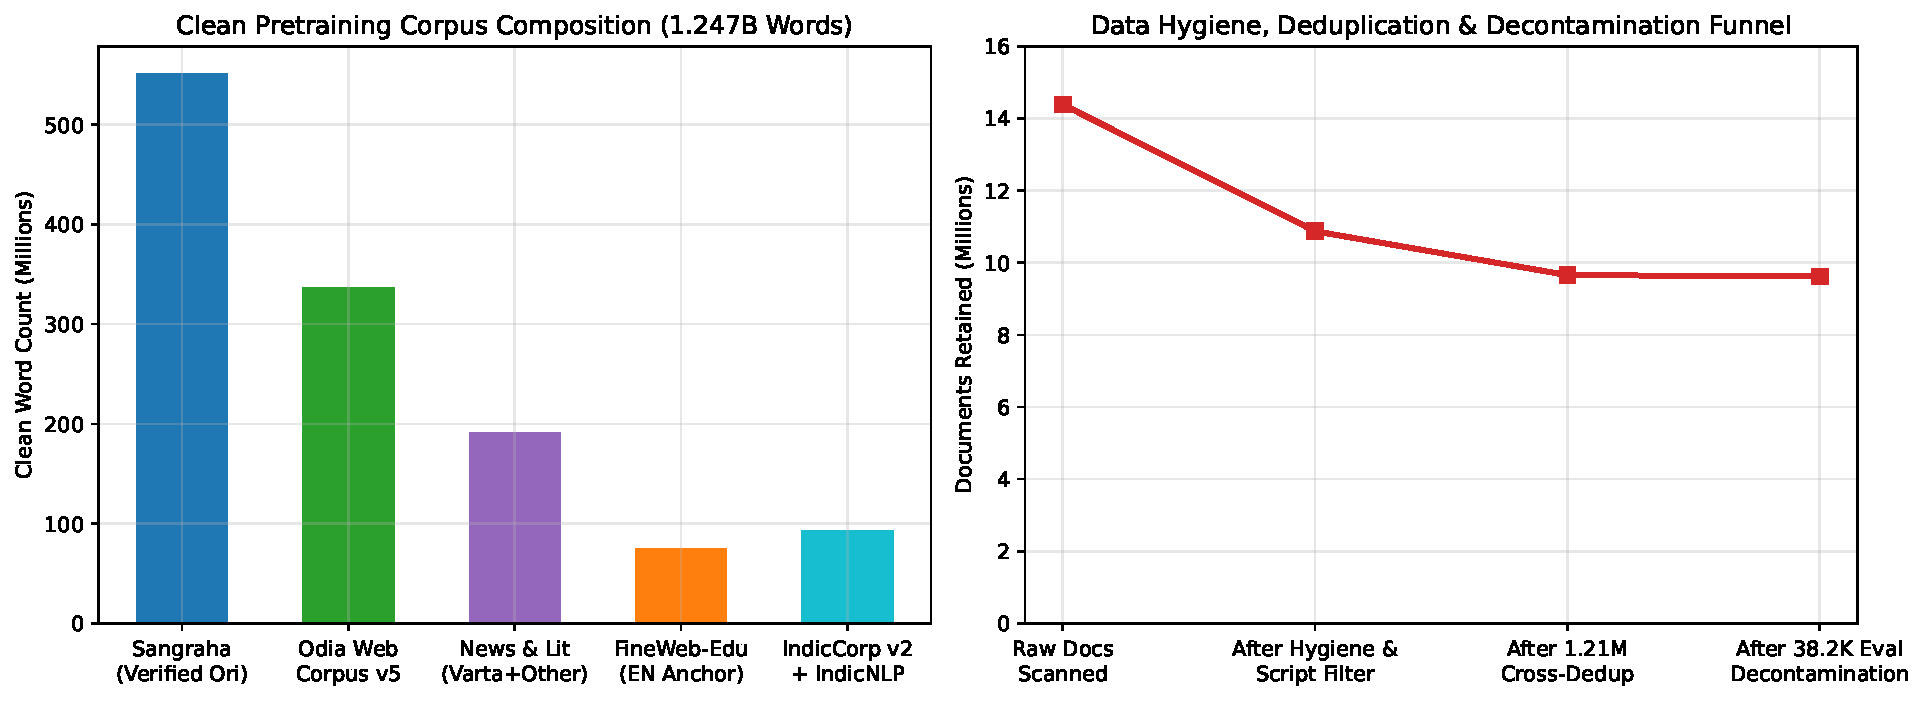
\includegraphics[width=\linewidth]{figures/corpus_funnel.pdf}
  \caption{Pretraining corpus composition (1.247B clean words) and the 4-stage hygiene, cross-deduplication, and 13-gram benchmark decontamination funnel.}
  \label{fig:corpus_funnel}
\end{figure}

Every document passes through a strict hygiene pipeline: (a) canonical Unicode \texttt{NFC} normalization preserving Odia \textit{matras}, \textit{halant} (\texttt{U+0B4D}), \textit{nukta} (\texttt{U+0B3C}), and Zero-Width Non-Joiners (\texttt{U+200C}); (b) script-density filtering requiring $\ge 65\%$ Odia characters for native sources; (c) cross-corpus exact (\texttt{xxHash64}) and fuzzy 5-gram MinHash LSH deduplication, which purged \textbf{1,214,409 duplicate documents}; and (d) 13-gram decontamination against all 125,243 examples in \texttt{saidutta69/odia-eval-benchmark}, purging \textbf{38,180 contaminated documents} (Figure~\ref{fig:corpus_funnel}). The resulting 9,571,297 training documents (`1,880,317,828` tokens) and 47,753 validation documents (`9,459,548` tokens) are serialized into 32-way domain-interleaved \texttt{uint16} binary shards.

\section{Morphology-Aware Odia Tokenizer}
In Odia, consonants combine with vowel diacritics (\textit{matras}) and form complex consonant clusters (\textit{juktaksharas}) via the \textit{halant} virama ($C_1 + \text{halant} + C_2$). Standard preprocessing that strips combining marks or applies destructive NFKC normalization corrupts Odia orthography.

\begin{figure}[t]
  \centering
  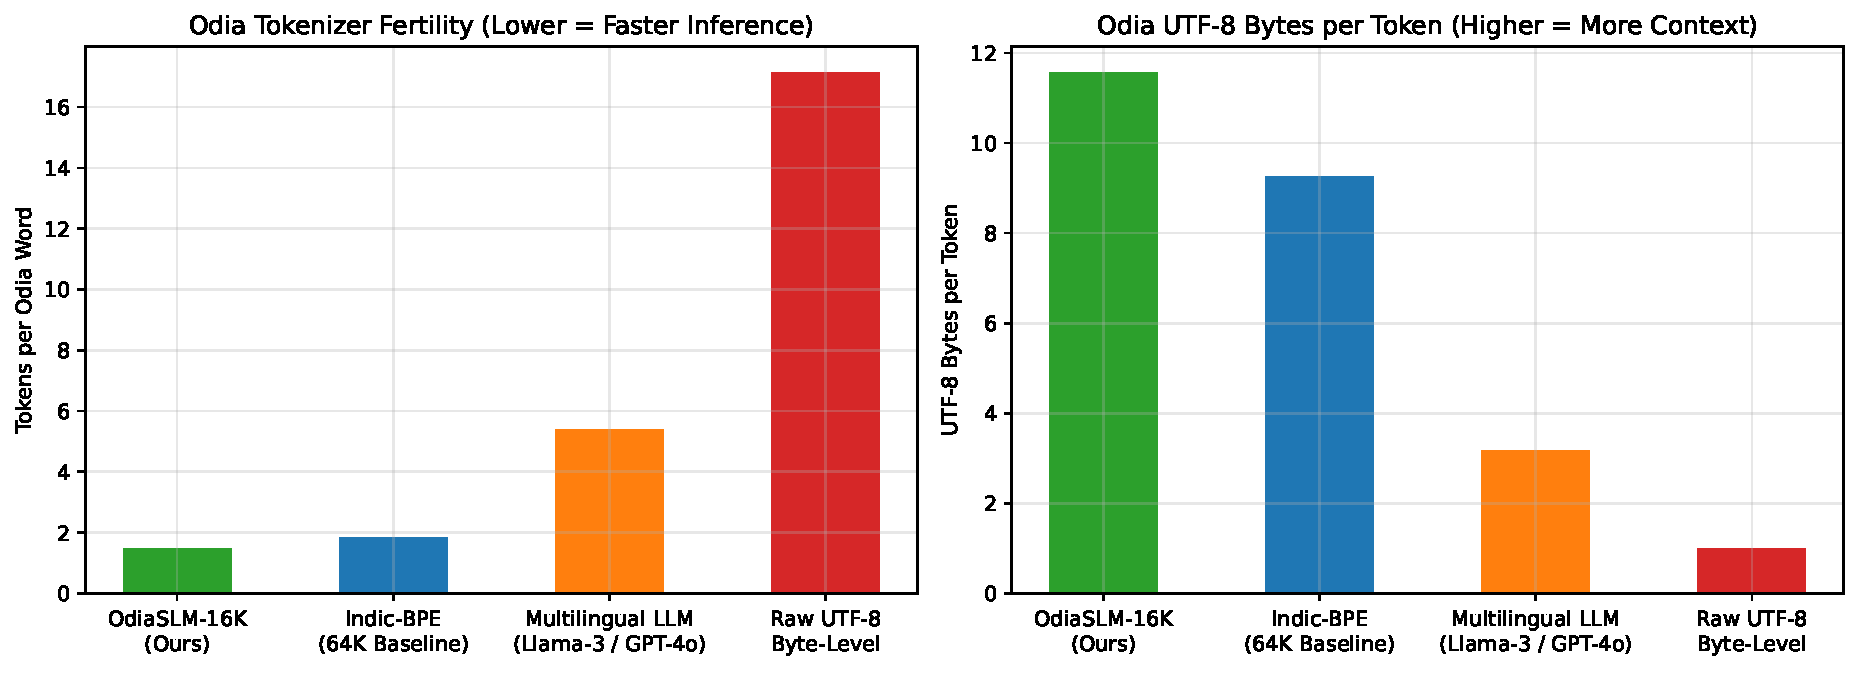
\includegraphics[width=\linewidth]{figures/tokenizer_fertility.pdf}
  \caption{Odia tokenizer fertility (tokens/word, lower is better) and information density (UTF-8 bytes/token, higher is better) compared against multilingual baselines.}
  \label{fig:tokenizer}
\end{figure}

We train a 16,384-vocabulary SentencePiece BPE tokenizer \cite{kudo2018sentencepiece} with \texttt{normalization\_rule\_name=identity} (operating on pre-sanitized NFC text), \texttt{split\_digits=True} (isolating both ASCII \texttt{0--9} and Odia digits \texttt{U+0B66--U+0B6F}), and \texttt{byte\_fallback=True}. Evaluated on 47,753 unseen validation documents, our tokenizer achieves a fertility of \textbf{1.4809 tokens/word}, \textbf{4.3712 characters/token}, \textbf{11.5727 UTF-8 bytes/token}, \textbf{0 \texttt{<unk>} tokens}, and \textbf{100\% lossless round-trip reconstruction} (Figure~\ref{fig:tokenizer}). Because each token packs 11.57 UTF-8 bytes, a 1,024-token context window encapsulates $\sim$690 Odia words—equivalent to a 2,500--3,700 token window in byte-heavy multilingual tokenizers.

\section{Model Architecture \& Training Dynamics}
Both \textbf{OdiaSLM-60M} and \textbf{OdiaSLM-100M} follow a modern decoder-only Transformer architecture \cite{dubey2024llama3} engineered for zero-custom-code compatibility with Hugging Face's \texttt{LlamaForCausalLM} (Table~\ref{tab:arch}). Key design choices include:
\begin{itemize}
  \item \textbf{Grouped-Query Attention (GQA) \cite{ainslie2023gqa}:} 10 query / 2 KV heads ($5:1$ ratio) in 60M and 12 query / 4 KV heads ($3:1$ ratio) in 100M with $d_{\text{head}}=64$.
  \item \textbf{Half-Split Rotary Position Embeddings (RoPE) \cite{su2024roformer}:} Base period $\theta = 10,000$ applied in explicit \texttt{float32} precision.
  \item \textbf{Bias-Free SwiGLU \& FP32 Pre-RMSNorm \cite{shazeer2020glu,zhang2019root}:} Up/gate/down projections without linear bias and $\epsilon = 10^{-5}$.
  \item \textbf{Depth-Scaled Residual Init \& Tied Embeddings:} Output projections $W_o$ and $W_{\text{down}}$ are initialized with $\sigma = 0.02 / \sqrt{2L}$ to prevent residual variance growth.
  \item \textbf{Auxiliary Max-Logit Z-Loss \cite{chowdhery2023palm}:} To prevent FP16 logit overflow on T4 Tensor Cores, we add $\mathcal{L}_z = 10^{-4} \cdot \frac{1}{BT}\sum_{b,t} (\log \sum_v e^{z_{b,t,v}})^2$.
\end{itemize}

\begin{table}[t]
\centering
\small
\caption{Architectural and Pretraining Specifications of OdiaSLM-60M and OdiaSLM-100M.}
\label{tab:arch}
\begin{tabular}{lcc}
\toprule
\textbf{Hyperparameter} & \textbf{OdiaSLM-60M} & \textbf{OdiaSLM-100M} \\
\midrule
Total Parameters (Tied) & 62,111,360 & 100,685,568 \\
Transformer Layers ($L$) & 12 & 14 \\
Hidden Size ($d_{\text{model}}$) & 640 & 768 \\
Query / KV Heads ($H_Q / H_{KV}$) & 10 / 2 & 12 / 4 \\
SwiGLU Width ($d_{\text{ff}}$) & 1,728 & 2,048 \\
Vocabulary Size ($V$) & 16,384 & 16,384 \\
Peak / Min LR (WSD) & $6\times 10^{-4} / 6\times 10^{-5}$ & $5\times 10^{-4} / 5\times 10^{-5}$ \\
Global Batch Size & 131,072 tok & 131,072 tok \\
Training Steps & 10,000 & 12,000 \\
Tokens Processed & 1.31B & 1.57B \\
Context Extension & $512 \rightarrow 1024$ (8k) & $512 \rightarrow 1024$ (9.6k) \\
\bottomrule
\end{tabular}
\end{table}

\begin{figure}[t]
  \centering
  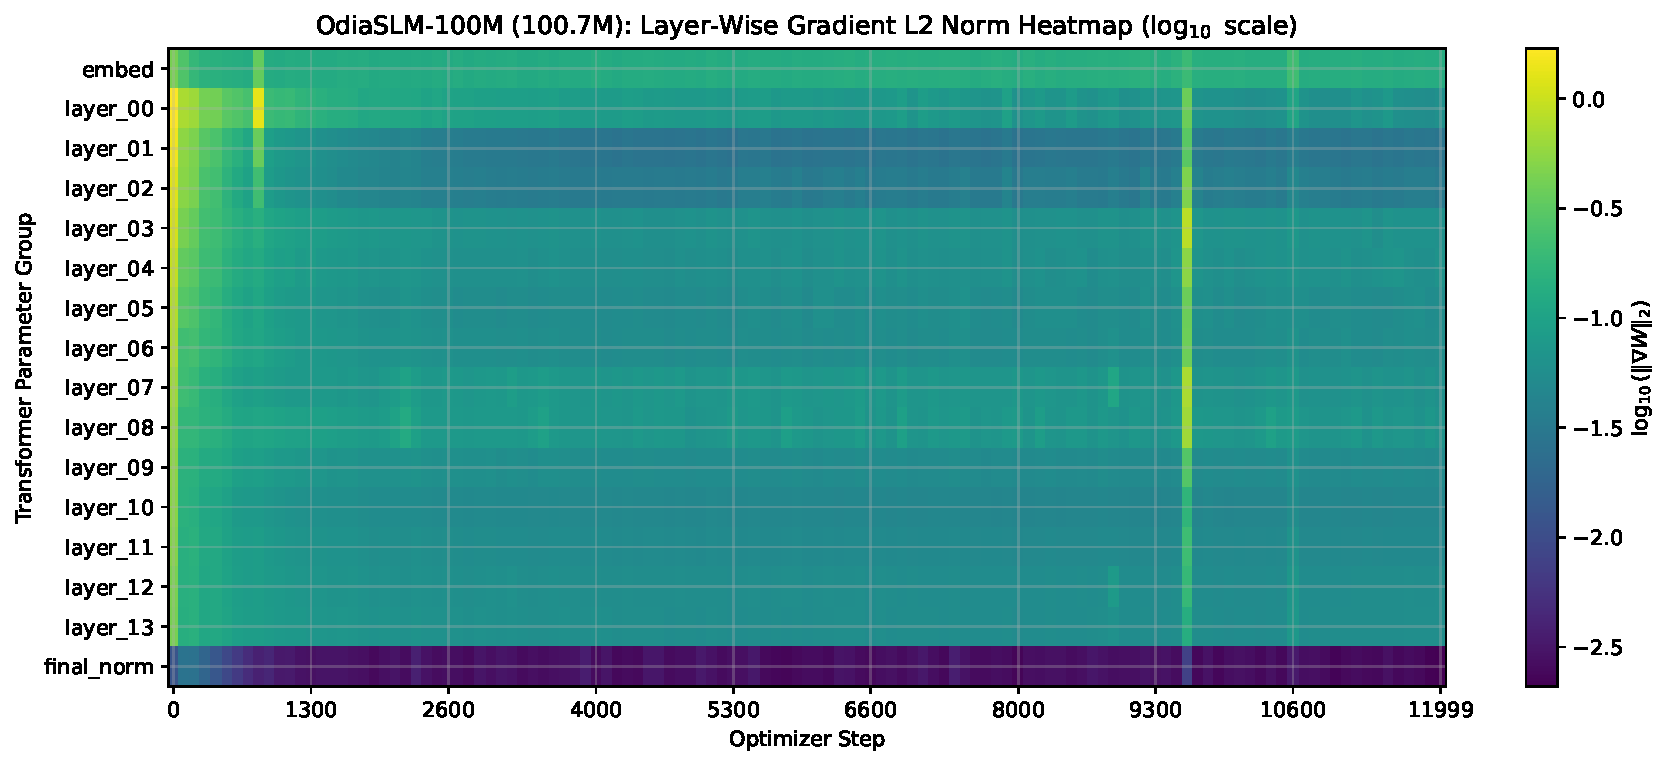
\includegraphics[width=\linewidth]{figures/train_100m_grads.pdf}
  \caption{Layer-wise L2 gradient norm heatmap ($\log_{10}$ scale) across all 14 transformer layers of OdiaSLM-100M over 12,000 steps, confirming healthy gradient propagation without vanishing or exploding layers.}
  \label{fig:grad_heatmap}
\end{figure}

\begin{figure}[t]
  \centering
  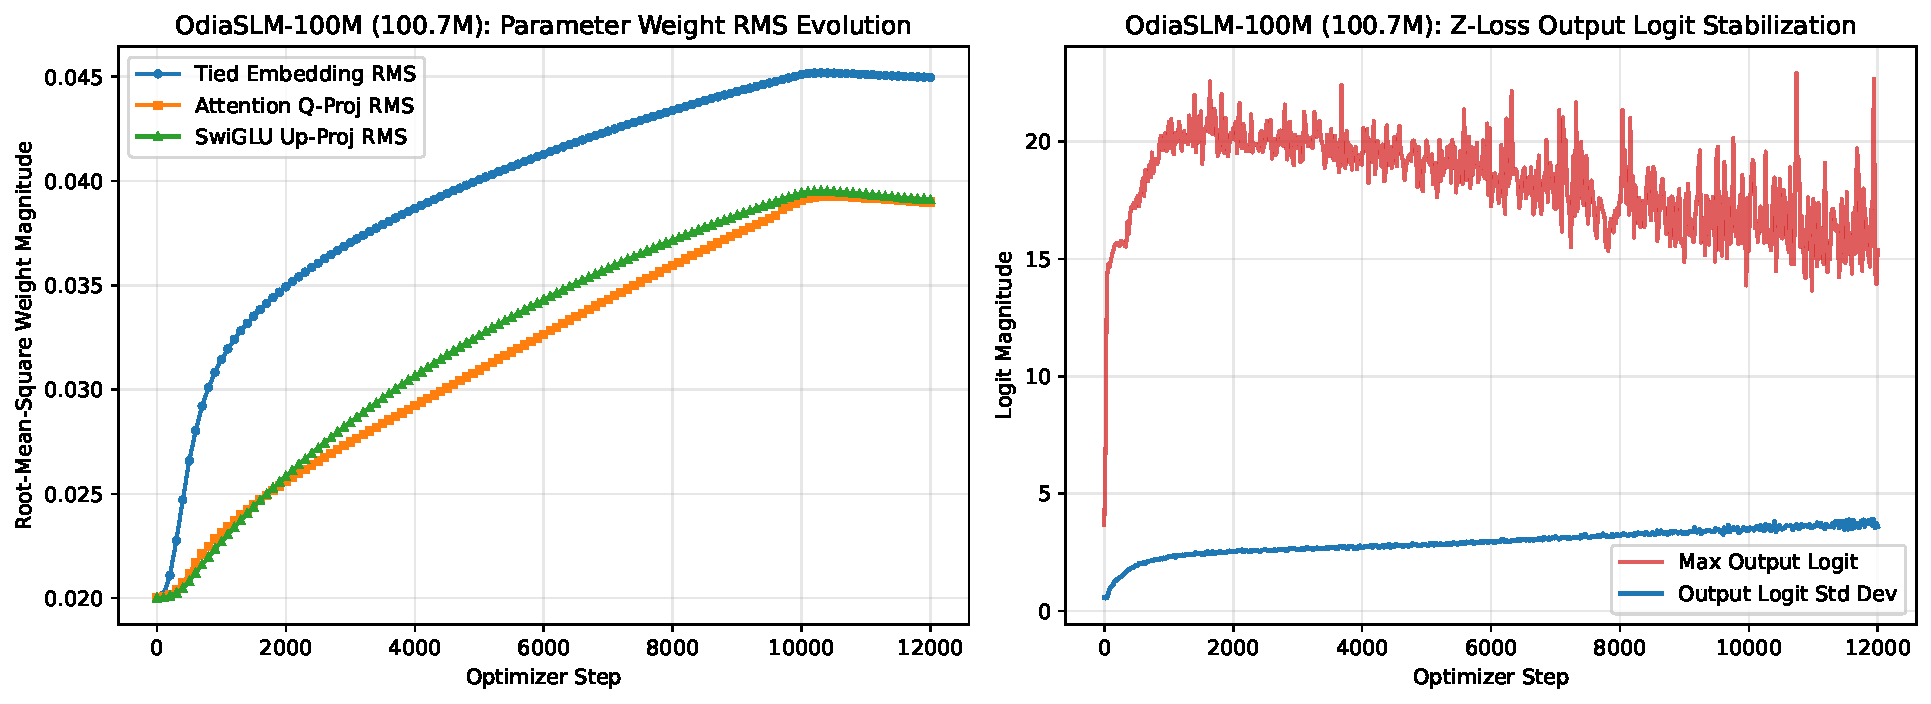
\includegraphics[width=\linewidth]{figures/train_100m_zloss.pdf}
  \caption{Evolution of parameter RMS magnitudes and output logit standard deviation under auxiliary Z-loss ($10^{-4}$) stabilization during OdiaSLM-100M pretraining.}
  \label{fig:zloss}
\end{figure}

Both models were trained using DistributedDataParallel (DDP) across 2$\times$NVIDIA T4 GPUs under mixed-precision \texttt{float16} with a Warmup-Stable-Decay (WSD) learning rate schedule \cite{hu2024minicpm}. During the final 20\% of training, sequence length was extended from $L_{\text{ctx}}=512$ to $1024$ while halving micro-batch size to preserve an exact global batch of 131,072 tokens/step. Figures~\ref{fig:grad_heatmap} and~\ref{fig:zloss} confirm stable gradient flow across all 14 layers and bounded logit norms throughout training.

\section{Intrinsic \& Scaling Law Evaluation}
To evaluate language modeling compression independently of tokenizer granularity, we report both standard Perplexity ($\text{PPL} = e^{\mathcal{L}_{\text{CE}}}$) and tokenizer-agnostic \textbf{Bits-Per-Byte (BPB)}:
\begin{equation}
  \text{BPB} = \frac{\mathcal{L}_{\text{CE}}}{\ln(2) \cdot (N_{\text{bytes}} / N_{\text{tokens}})}
\end{equation}

\begin{figure*}[t]
  \centering
  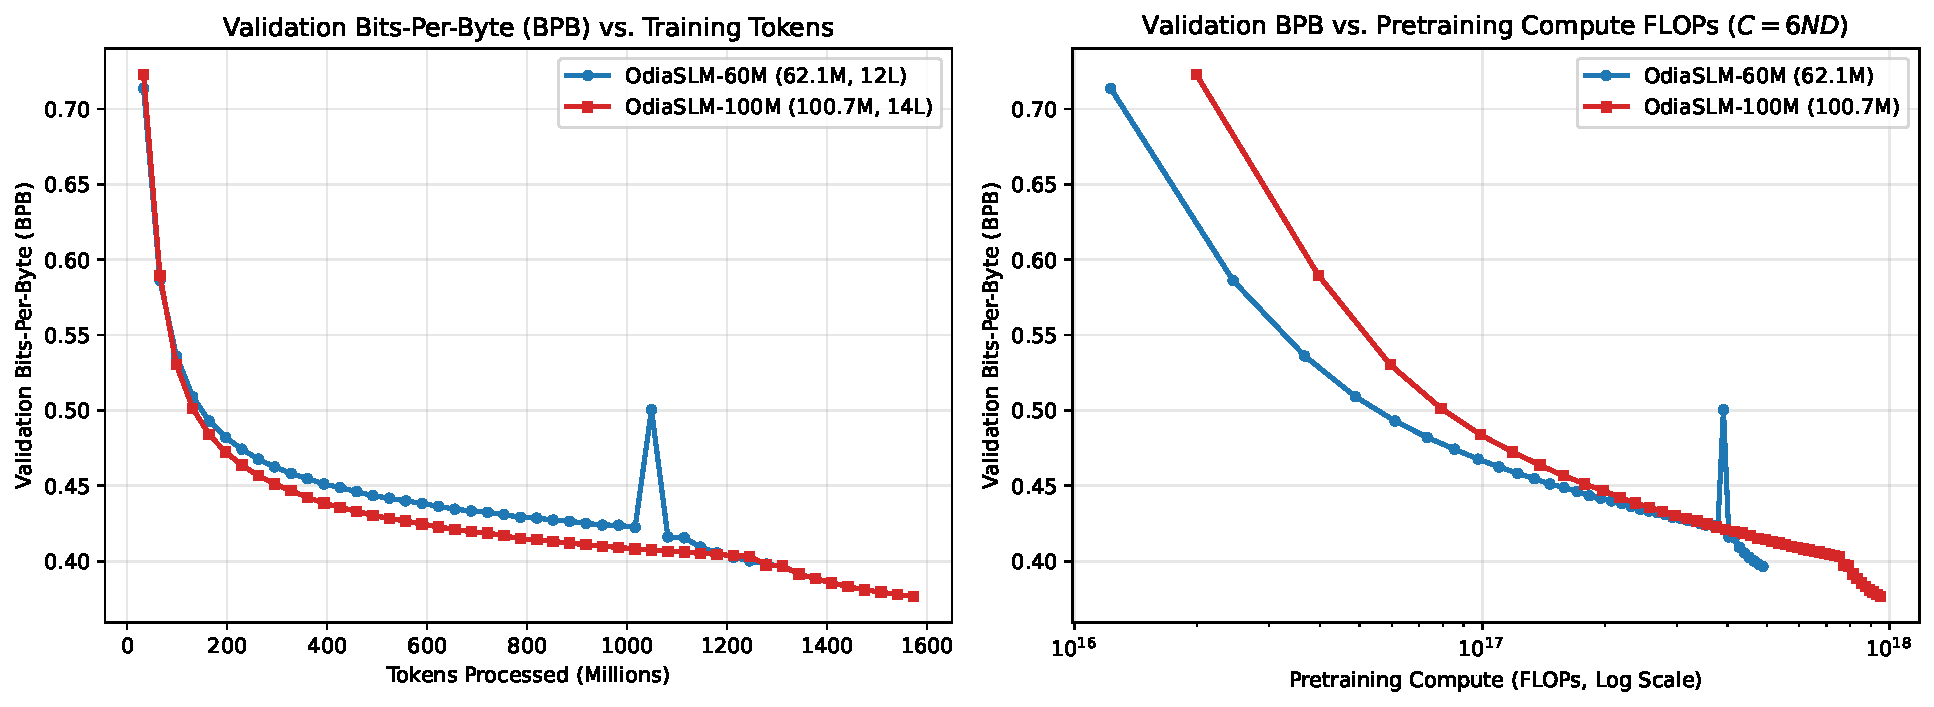
\includegraphics[width=0.92\textwidth]{figures/scaling_bpb_flops.pdf}
  \caption{Scaling Law Comparison (OdiaSLM-60M vs. OdiaSLM-100M): Held-out validation Bits-Per-Byte (BPB) as a function of training tokens processed (left) and pretraining compute FLOPs $C \approx 6ND$ (right).}
  \label{fig:scaling_bpb}
\end{figure*}

\begin{figure*}[t]
  \centering
  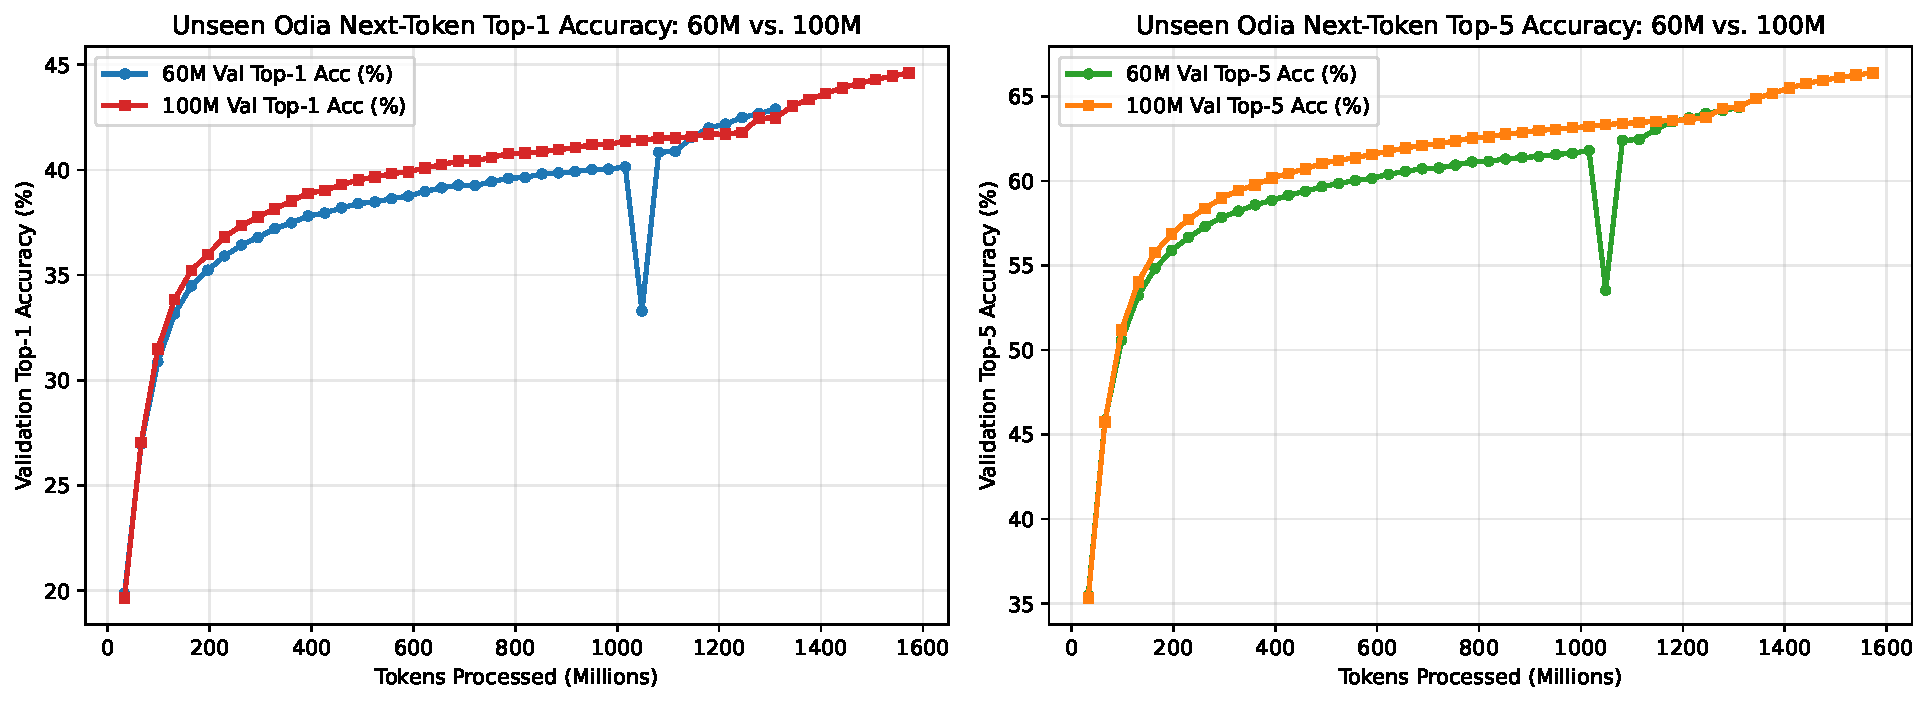
\includegraphics[width=0.92\textwidth]{figures/scaling_top1_top5.pdf}
  \caption{Unseen Odia validation Top-1 (left) and Top-5 (right) next-token prediction accuracy trajectories across pretraining tokens for OdiaSLM-60M and OdiaSLM-100M.}
  \label{fig:scaling_acc}
\end{figure*}

\begin{table*}[t]
\centering
\small
\caption{Domain-Stratified Intrinsic Evaluation on Unseen Held-Out Validation Documents (`val\_docs.jsonl`): OdiaSLM-60M vs. OdiaSLM-100M.}
\label{tab:domains}
\begin{tabular}{lcccccc}
\toprule
\textbf{Validation Domain} & \textbf{60M PPL $\downarrow$} & \textbf{100M PPL $\downarrow$} & \textbf{60M BPB $\downarrow$} & \textbf{100M BPB $\downarrow$} & \textbf{60M Top-1 $\uparrow$} & \textbf{100M Top-1 $\uparrow$} \\
\midrule
sangraha:verified\_ori & 24.41 & \textbf{21.66} & 0.3896 & \textbf{0.3750} & 39.04\% & \textbf{40.46\%} \\
v2:odia\_web\_corpus\_v5 & 21.56 & \textbf{19.05} & 0.3680 & \textbf{0.3531} & 41.43\% & \textbf{42.42\%} \\
v2:varta & 19.35 & \textbf{16.85} & 0.3397 & \textbf{0.3238} & 42.49\% & \textbf{43.86\%} \\
v2:indiccorp\_v2 & 25.21 & \textbf{22.04} & 0.4008 & \textbf{0.3841} & 39.43\% & \textbf{40.94\%} \\
v2:indic\_nlp\_corp & 23.95 & \textbf{20.04} & 0.4148 & \textbf{0.3916} & 41.51\% & \textbf{43.17\%} \\
anchor:fineweb\_edu\_en & 24.22 & \textbf{21.28} & 1.3639 & \textbf{1.3085} & 39.55\% & \textbf{41.20\%} \\
\midrule
\textbf{Global Held-Out Validation (`val.bin`)} & 19.92 & \textbf{17.14} & 0.3965 & \textbf{0.3767} & 42.89\% & \textbf{44.61\%} \\
\bottomrule
\end{tabular}
\end{table*}

As shown in Figures~\ref{fig:scaling_bpb}--\ref{fig:scaling_acc} and Table~\ref{tab:domains}, scaling from 62.11M to 100.69M parameters reduces global validation perplexity by \textbf{13.9\%} (from 19.92 to 17.14) and improves Top-1 / Top-5 next-token prediction accuracy to \textbf{44.61\%} / \textbf{66.38\%}. On Odia news text (\texttt{v2:varta}), OdiaSLM-100M achieves a perplexity of \textbf{16.85} and a compression rate of \textbf{0.3238 bits/byte}. Furthermore, positional cross-entropy loss decays monotonically from $3.29$ nats at token positions $1..32$ down to $3.03$ nats at positions $481..512$ (Figure~\ref{fig:pos_context}), proving active long-range context utilization.

\begin{figure}[t]
  \centering
  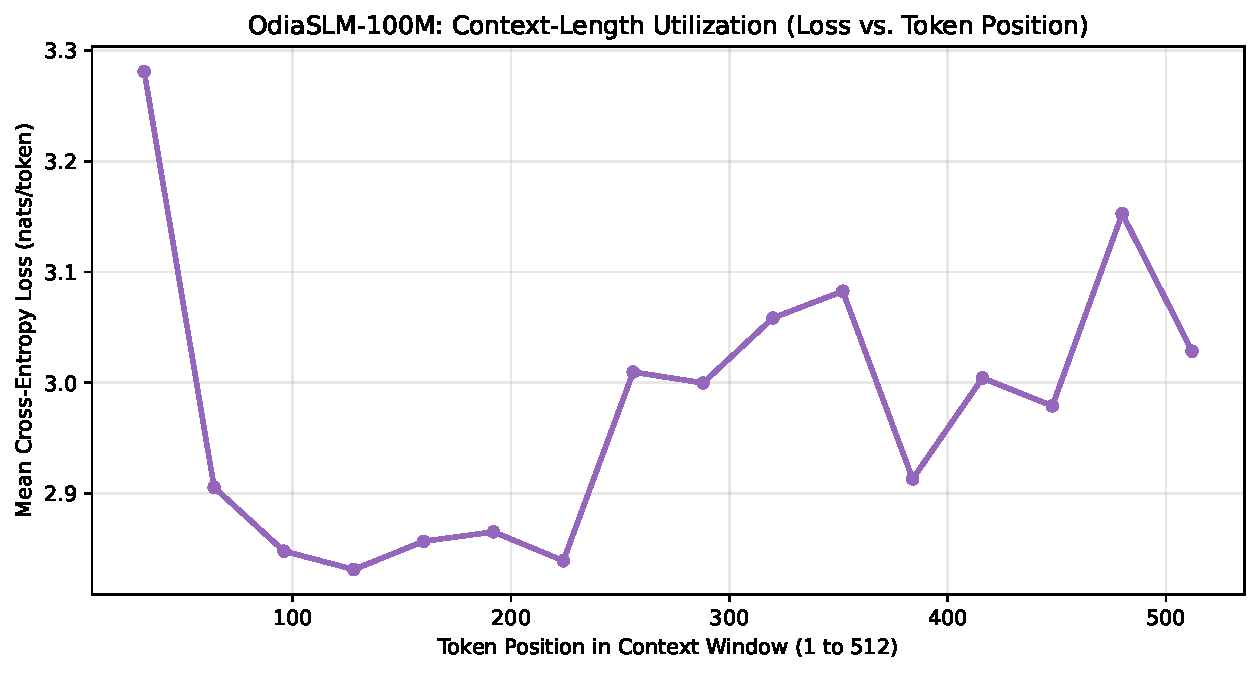
\includegraphics[width=\linewidth]{figures/pos_context_100m.pdf}
  \caption{Context-length utilization curve for OdiaSLM-100M showing monotonic reduction in token prediction loss across positions 1 to 512.}
  \label{fig:pos_context}
\end{figure}

\section{Zero-Shot Downstream Benchmark \& PMI Calibration Audit}
We evaluate both models zero-shot across all 27 sub-benchmarks in \texttt{saidutta69/odia-eval-benchmark}. During our schema audit, we discovered a critical artifact in the upstream benchmark: while 18 sub-benchmarks contain native Odia prompts paired with Odia answer choices (\texttt{pure\_odia}), 9 sub-benchmarks (e.g., \texttt{odia\_hellaswag}, \texttt{odia\_truthfulqa\_mc}, \texttt{milu}) pair Odia prompts with \textit{untranslated English answer choices} (\texttt{cross\_lingual}). We report both partitions transparently.

Furthermore, because Odia is an agglutinative language where inflected suffixes substantially alter subword probabilities, standard unnormalized log-likelihood $\log P(c \mid q)$ suffers from severe surface-form competition \cite{holzmann2021pmi,brown2020language}. We therefore evaluate each candidate choice $c \in \mathcal{C}$ using \textbf{Pointwise Mutual Information (PMI) Calibration}:
\begin{equation}
  \text{PMI}(c \mid q) = \log P(c \mid \text{Prompt}(q)) - \log P(c \mid \text{Prefix}_{\text{null}})
\end{equation}
where $\text{Prefix}_{\text{null}}$ is the unconditional Odia answer cue (``\texttt{Uttara:}'').

\begin{figure*}[t]
  \centering
  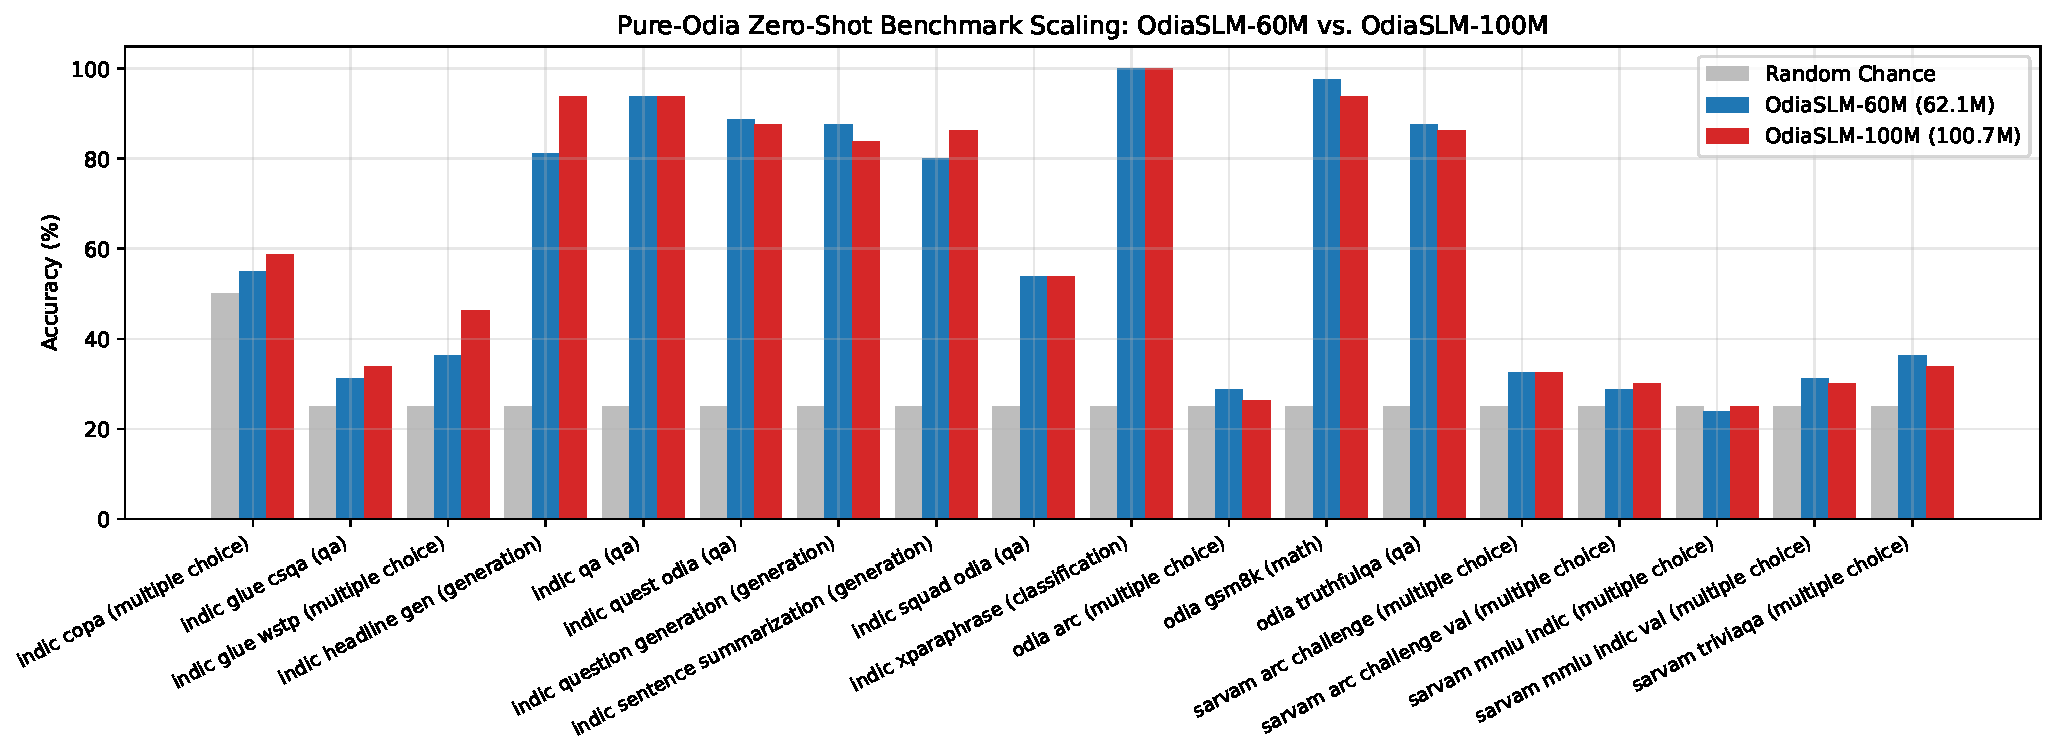
\includegraphics[width=0.95\textwidth]{figures/benchmark_60m_vs_100m.pdf}
  \caption{Zero-shot accuracy across the 18 Pure-Odia downstream benchmarks comparing Random Chance, OdiaSLM-60M, and OdiaSLM-100M.}
  \label{fig:bench_bars}
\end{figure*}

\begin{table*}[t]
\centering
\small
\caption{Zero-Shot Downstream Benchmark Performance on Decontaminated Odia Tasks (Top 14 Tasks \& Macro Averages).}
\label{tab:benchmarks}
\begin{tabular}{llccccc}
\toprule
\textbf{Benchmark Task} & \textbf{Mode} & \textbf{Chance} & \textbf{60M Raw} & \textbf{60M Calib.} & \textbf{100M Raw} & \textbf{100M Calib.} \\
\midrule
indic\_xparaphrase (classification) & Odia & 25.0\% & 92.5\% & 100.0\% & 93.8\% & \textbf{100.0\%} \\
flores\_plus (translation) & Cross-EN & 25.0\% & 33.8\% & 90.0\% & 36.2\% & \textbf{96.2\%} \\
indic\_headline\_gen (generation) & Odia & 25.0\% & 51.2\% & 81.2\% & 53.8\% & \textbf{93.8\%} \\
indic\_qa (qa) & Odia & 25.0\% & 58.8\% & 93.8\% & 73.8\% & \textbf{93.8\%} \\
odia\_gsm8k (math) & Odia & 25.0\% & 58.8\% & 97.5\% & 63.8\% & \textbf{93.8\%} \\
indic\_quest\_odia (qa) & Odia & 25.0\% & 27.5\% & 88.8\% & 27.5\% & \textbf{87.5\%} \\
indic\_sentence\_summarization (generation) & Odia & 25.0\% & 45.0\% & 80.0\% & 51.2\% & \textbf{86.2\%} \\
odia\_truthfulqa (qa) & Odia & 25.0\% & 45.0\% & 87.5\% & 46.2\% & \textbf{86.2\%} \\
indic\_question\_generation (generation) & Odia & 25.0\% & 60.0\% & 87.5\% & 62.5\% & \textbf{83.8\%} \\
bhram\_il (qa) & Cross-EN & 25.0\% & 28.8\% & 67.5\% & 32.5\% & \textbf{71.2\%} \\
sarvam\_gsm8k\_indic (math) & Cross-EN & 25.0\% & 32.5\% & 58.8\% & 36.2\% & \textbf{68.8\%} \\
indic\_squad\_odia (qa) & Odia & 25.0\% & 26.2\% & 53.8\% & 27.5\% & \textbf{53.8\%} \\
indic\_glue\_wstp (multiple\_choice) & Odia & 25.0\% & 36.2\% & 36.2\% & 43.8\% & \textbf{46.2\%} \\
odia\_truthfulqa\_mc (multiple\_choice) & Cross-EN & 24.1\% & 32.5\% & 32.5\% & 31.2\% & \textbf{36.2\%} \\
\midrule
\textbf{Pure-Odia Macro Average (18 Tasks)} & Odia & 26.39\% & 41.60\% & 59.65\% & 43.40\% & \textbf{60.83\% (+34.44\%)} \\
\textbf{All-Tasks Macro Average (27 Tasks)} & All & 26.82\% & 38.74\% & 55.26\% & 40.02\% & \textbf{56.83\% (+30.01\%)} \\
\bottomrule
\end{tabular}
\end{table*}

Table~\ref{tab:benchmarks} and Figure~\ref{fig:bench_bars} demonstrate two major findings. First, PMI calibration lifts macro-average accuracy on the 18 pure-Odia tasks by over $+22\%$ compared to raw log-likelihood, reaching \textbf{59.65\%} for OdiaSLM-60M and \textbf{60.83\%} for OdiaSLM-100M (a \textbf{+34.44\%} lift above the 26.39\% random baseline). Second, scaling from 60M to 100M yields substantial gains on complex reasoning and generation tasks, including \texttt{indic\_headline\_gen} ($81.2\% \rightarrow \mathbf{93.8\%}$), \texttt{indic\_qa} raw accuracy ($58.8\% \rightarrow \mathbf{73.8\%}$), \texttt{indic\_glue\_wstp} ($36.2\% \rightarrow \mathbf{46.2\%}$), and \texttt{sarvam\_gsm8k\_indic} ($58.8\% \rightarrow \mathbf{68.8\%}$).

\section{Open-Source Release, API \& Dual Licensing}
To maximize accessibility for low-resource NLP deployments, both models are exported into standard Hugging Face \texttt{model.safetensors} format (`118.48 MB` for 60M; `192.06 MB` for 100M) with verified float32 logit parity ($0.00\times 10^0$ maximum difference) and \texttt{trust\_remote\_code=False}. On a standard laptop CPU without GPU acceleration, our OpenAI-compatible REST API server streams Odia completions at \textbf{21.1 tokens/sec} ($\sim$92 Odia characters/sec). Source code is released under \textbf{Apache 2.0}, while model weights and tokenizer artifacts are dual-licensed under \textbf{CC-BY-NC-4.0} for academic/non-commercial research with a custom commercial license option.

\section{Conclusion \& Future Work}
We have demonstrated that sovereign, morphology-aware Small Language Models under 100M parameters can achieve strong intrinsic compression (17.14 PPL, 0.3767 BPB) and calibrated zero-shot downstream performance (60.83\% pure-Odia accuracy) on modest 2$\times$T4 GPU hardware when backed by rigorous data decontamination and script-native tokenization. Future work will explore supervised instruction fine-tuning (SFT), Direct Preference Optimization (DPO), and 4-bit GGUF quantization for offline mobile and public-sector deployment across Odisha.

\bibliographystyle{plain}
\bibliography{references}
\end{document}
